\documentclass[12pt]{article}

\usepackage{graphicx}
\usepackage[margin=1.0in]{geometry}
\usepackage{amsmath}
\usepackage{cases}
\usepackage{amsfonts}
\usepackage{amssymb}
\usepackage{grffile}
\usepackage{setspace}

\setlength\parindent{0pt}

\author{Xiaohui Chen \\EID: xc2388}
\title{M 362K Pre-Class Work for 1/27}

\begin{document}
\maketitle
\begin{spacing}{2.0}

\section*{2-1}
\subsection*{(a)}
$O=\{1,3,5,7,9\}$, $P=\{2,3,5,7\}$

\subsection*{(b)}

$O\cap P = \{3,5,7\}$

\subsection*{(c)}

$O\cup P = \{1,2,3,5,7,9\}$

\subsection*{(d)}

$O-P=\{1,9\}$

\section*{2-6}

Let set $A=\{sum\ divisible\ by\ three\} = \{(1,2),(2,1),(1,5),(5,1),(2,4),(4,2),(3,3)\}$ and let $B= \{doubles\}= \{(1,1),(2,2),(3,3),(4,4),(5,5),(6,6)\} $

$\therefore Pr(A)=\frac{7}{36}$, $Pr(B)=\frac{6}{36}=\frac{1}{6}$ and $Pr(A \cap B)=\frac{1}{36}$

Using the inclusion-exclusion principle, we get $Pr(A\cup B)= Pr(A)+Pr(B)-Pr(A \cap B)= \frac{7+6-1}{36}=\frac{12}{36}= \frac{1}{3}$

\section*{2-8}

$A'=\{2,4,6,8,10\}$, $B'=\{1,4,6,8,9,10\}$, $A\cup B =\{1,2,3,5,7,9\}$, $A\cap B= \{3,5,7\},$

$A' \cup B'= \{1,2,3,4,6,8,9,10\}$, $A' \cap B'= \{4,6,8,10\}$, $(A\cup B)'= \{4,6,8,10\}$

\section*{2-18}
From the question, we know:

$N(U)=28$, $N(Adult)=18$, $N(Female)=13$, $N(Purple-hair)=11$,

$N(Adult\cap Female)=11$, $N(Adult\cap Female \cap Purple-hair)=6$, $N(Adult\cap Purple-hair)= 10$, $N(Female\cap Purple-hair=0)$

We want to calculate $N(Adult'\cap Purple-hair' \cap Female')$

\begin{figure}
  \centering
  % Requires \usepackage{graphicx}
  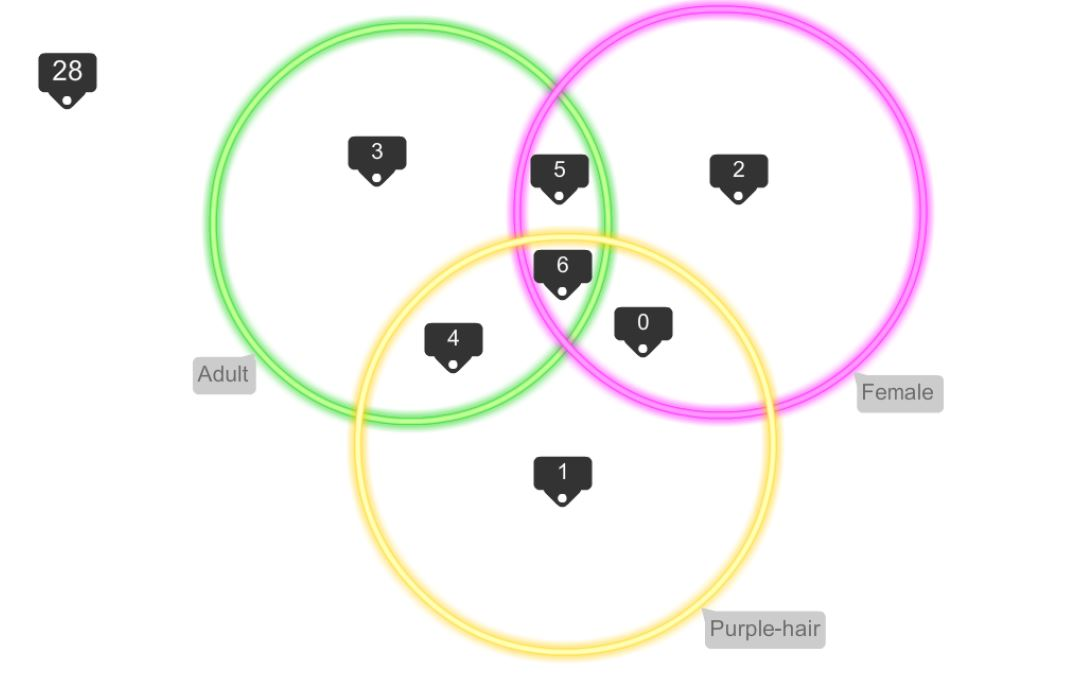
\includegraphics[width=6in]{venn}\\
  \caption{The Venn Diagram for the Family}\label{venn}
\end{figure}

The Venn diagram is shown in Figure \ref{venn}. According to the diagram, we can get that $N(Adult'\cap Purple-hair' \cap Female')= N(U)- N(Adult\cup Female\cup Purple-hair)= 28-(18+1+2)=7$

Therefore there are 7 male children without purple hair in the family

\end{spacing}
\end{document} 